\chapter{Background Material: on Convolutional Neural Networks}

\noindent We first start with a brief review of feedforward neural networks before elaborating on convolutional neural networks (CNNs). 

\section{Feed Forward Neural Networks}

A feedforward neural networks is a standard model in the machine literature for classification problems. It consists of a number of layers of simple processing units, also called neurons or nodes in which units in a layer are connected to units in the previous layers, each connection characterised by a weight encoding the knowledge of the network. Layers in which every unit is only connected to every unit in the previous layer are called fully-connected layers. The value at each unit is generated by taking a linear combination of the values of the incoming connections weighted by their weights and then passing the result through an activation function, such as a Rectified Linear or a Tanh function, serving as the output of that unit. Data enters at the input layer, passes through the network, layer by layer, until it arrives at the output layer. The choice of the activation function at the output layer is determined by the nature of the data and the assumed distribution of target variables. For classification problems, the softmax function or, in our case, its log, give the output a probabilistic interpretation.\\

\noindent This model can be represented in the form of a network diagram as shown in figure whatever. The process can then be interpreted as a forward propagation of information through the network.\\

\begin{figure}
\centering
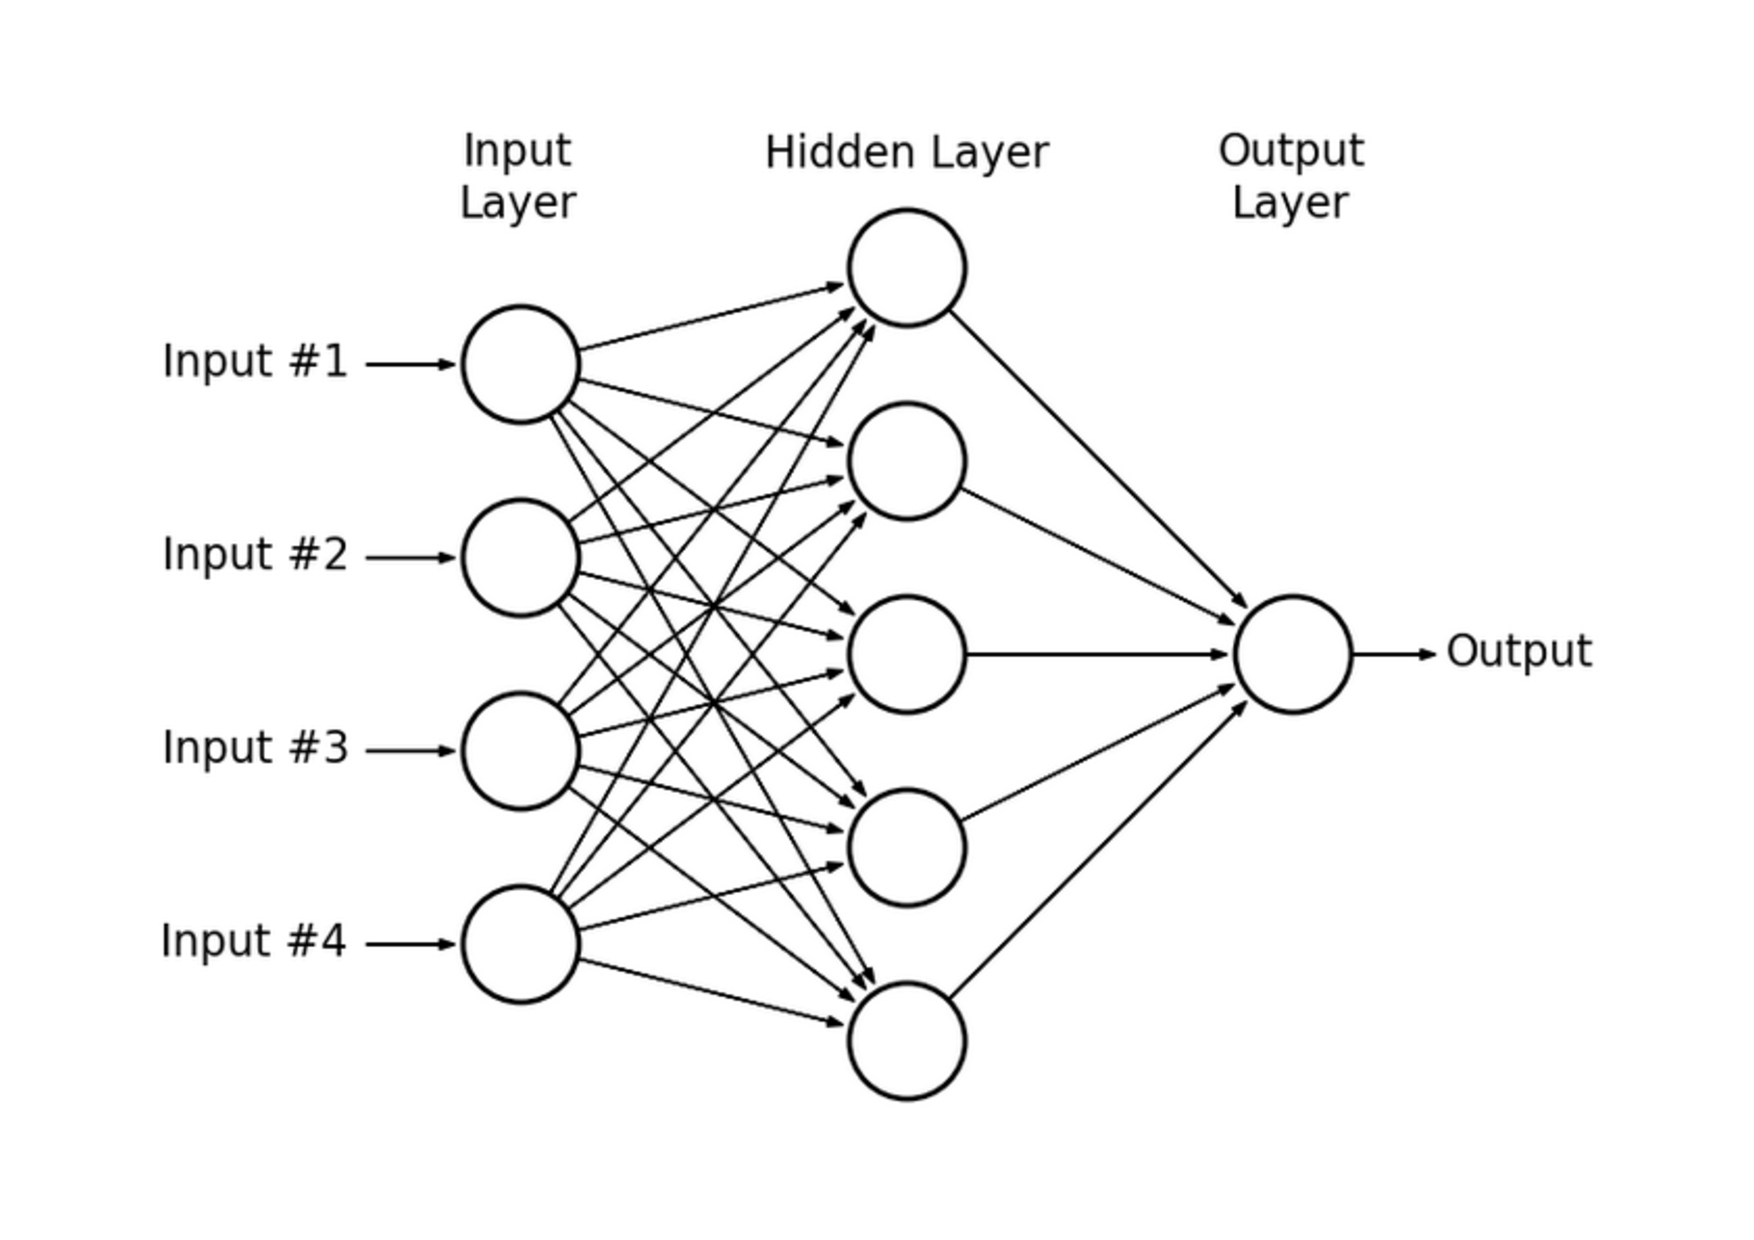
\includegraphics[trim=2cm 2cm 2cm 2cm, clip=true, height=80mm]{Chapter2/FF_Neural_Network.pdf}
%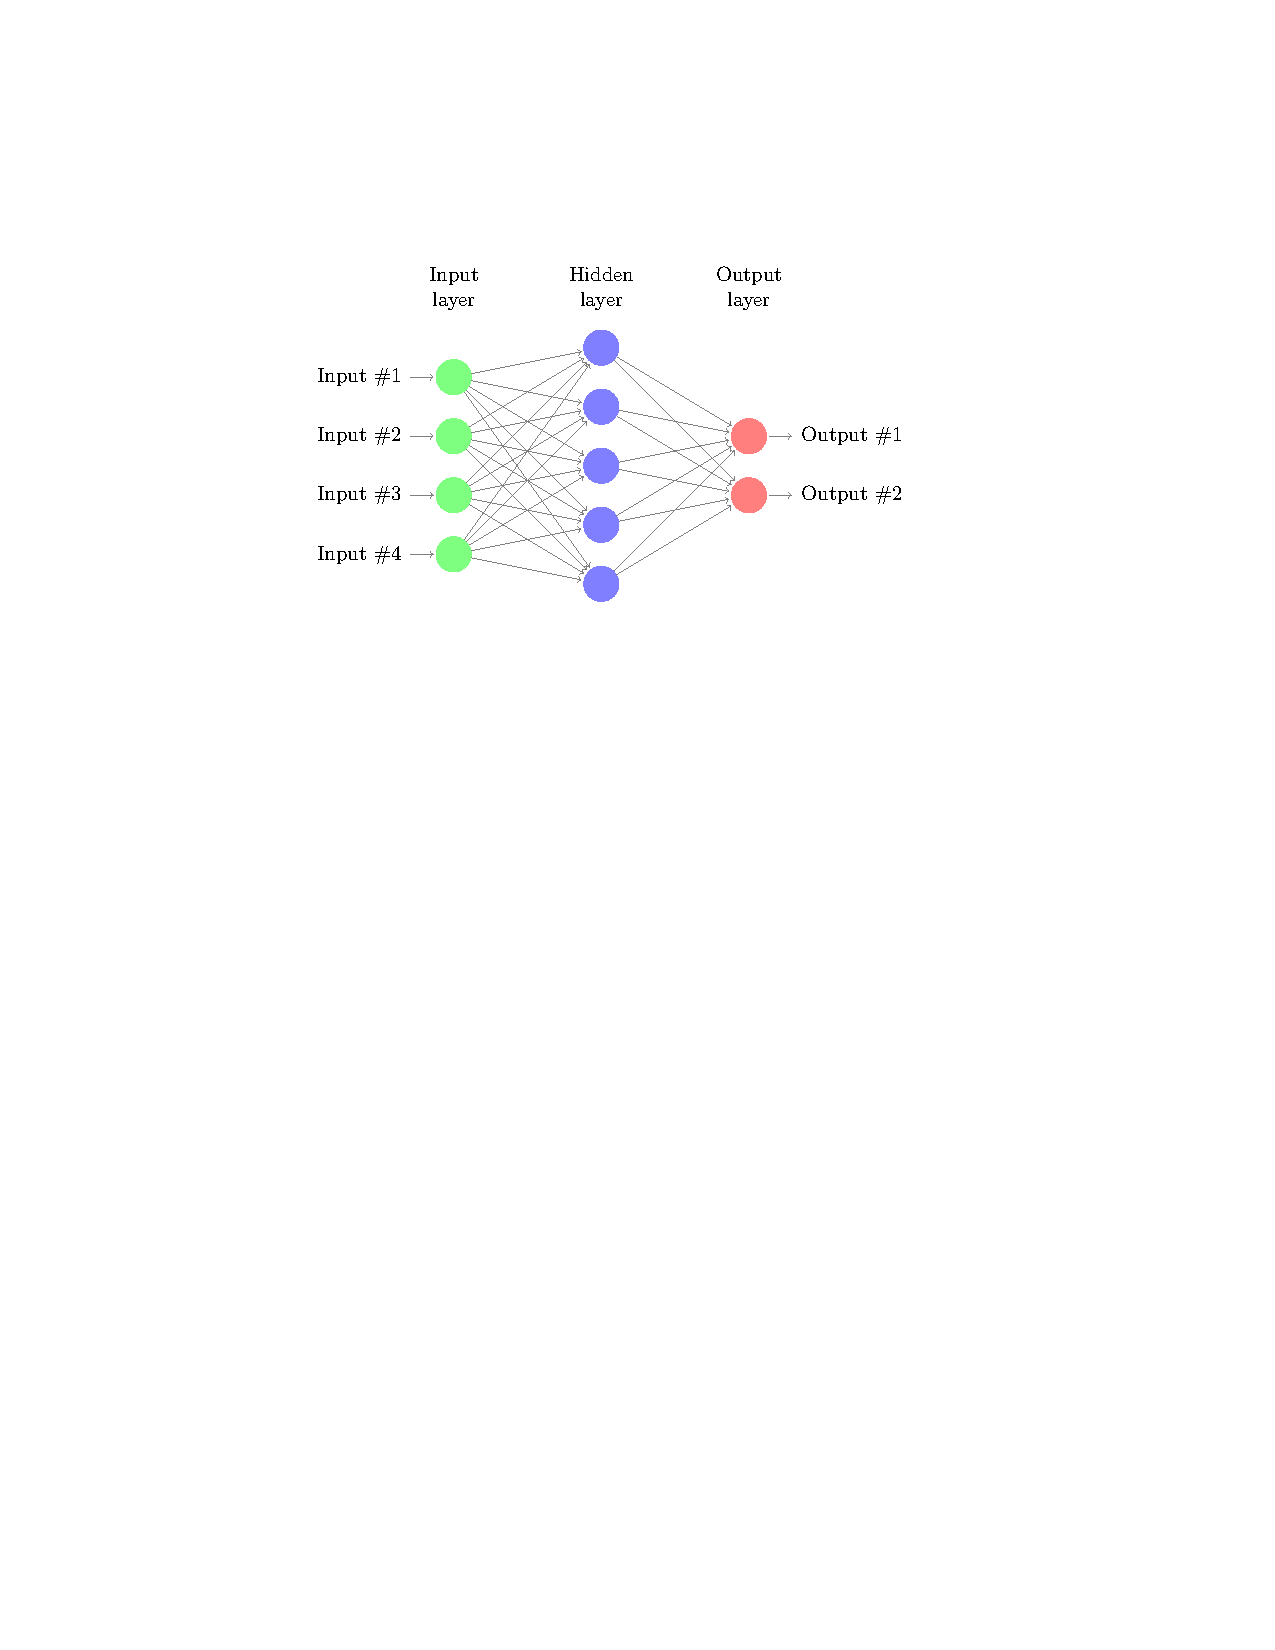
\includegraphics[trim=4cm 17cm 3cm 4cm, clip=true, height=80mm]{Tikz/NN.pdf}
\caption{A 2 layer feedforward neural network with 4 input nodes, 5 hidden nodes and 1 output node.}
\end{figure}

\noindent Training the neural networks is done by minimising an error measure of its performance over a training set using gradient-based optimisation routines. Evaluating the error gradients with respect to the parameters can be efficiently done via the backpropagation algorithm [reference]. Regularisation such as dropout [reference] where at every epoch, only a preset percentage of randomly chosen set of hidden units are active, is generally added to the optimisation procedure to prevent overfitting.

\section{Convolutional Layers}

\noindent A CNN is a specialised kind of feedforward neural network where the first few layers of the architecture are convolutional layers. These consist of three stages: a convolution stage, a detection stage and a subsampling stage. 

\subsection{Convolution}

\noindent The convolution stage is responsible for implementing $k$ convolution operations over each channel of the input images. This is accomplished by convolving each channel of the input layer with $k$ kernels of size $s \times s$ in parallel. Unlike fully connected layers, in a convolution, each output node is locally connected to a small contiguous subset of corresponding input nodes determined by the kernel size. Additionally the convolution operation implies weight sharing which greatly reduces the number of trainable parameters. In the case of $m \times m$ input images, the set of output nodes resulting from one kernel is called a feature map of size $(m - s/2 + 1) \times (m - s/2 + 1)$, each detecting the presence of a particular feature in the input image encoded by the kernel. Having multiple kernels run through the input layer in parallel produces a set of feature maps, each responsible for detecting a particular type of feature which might be present in the image. \\

\begin{figure}
\centering
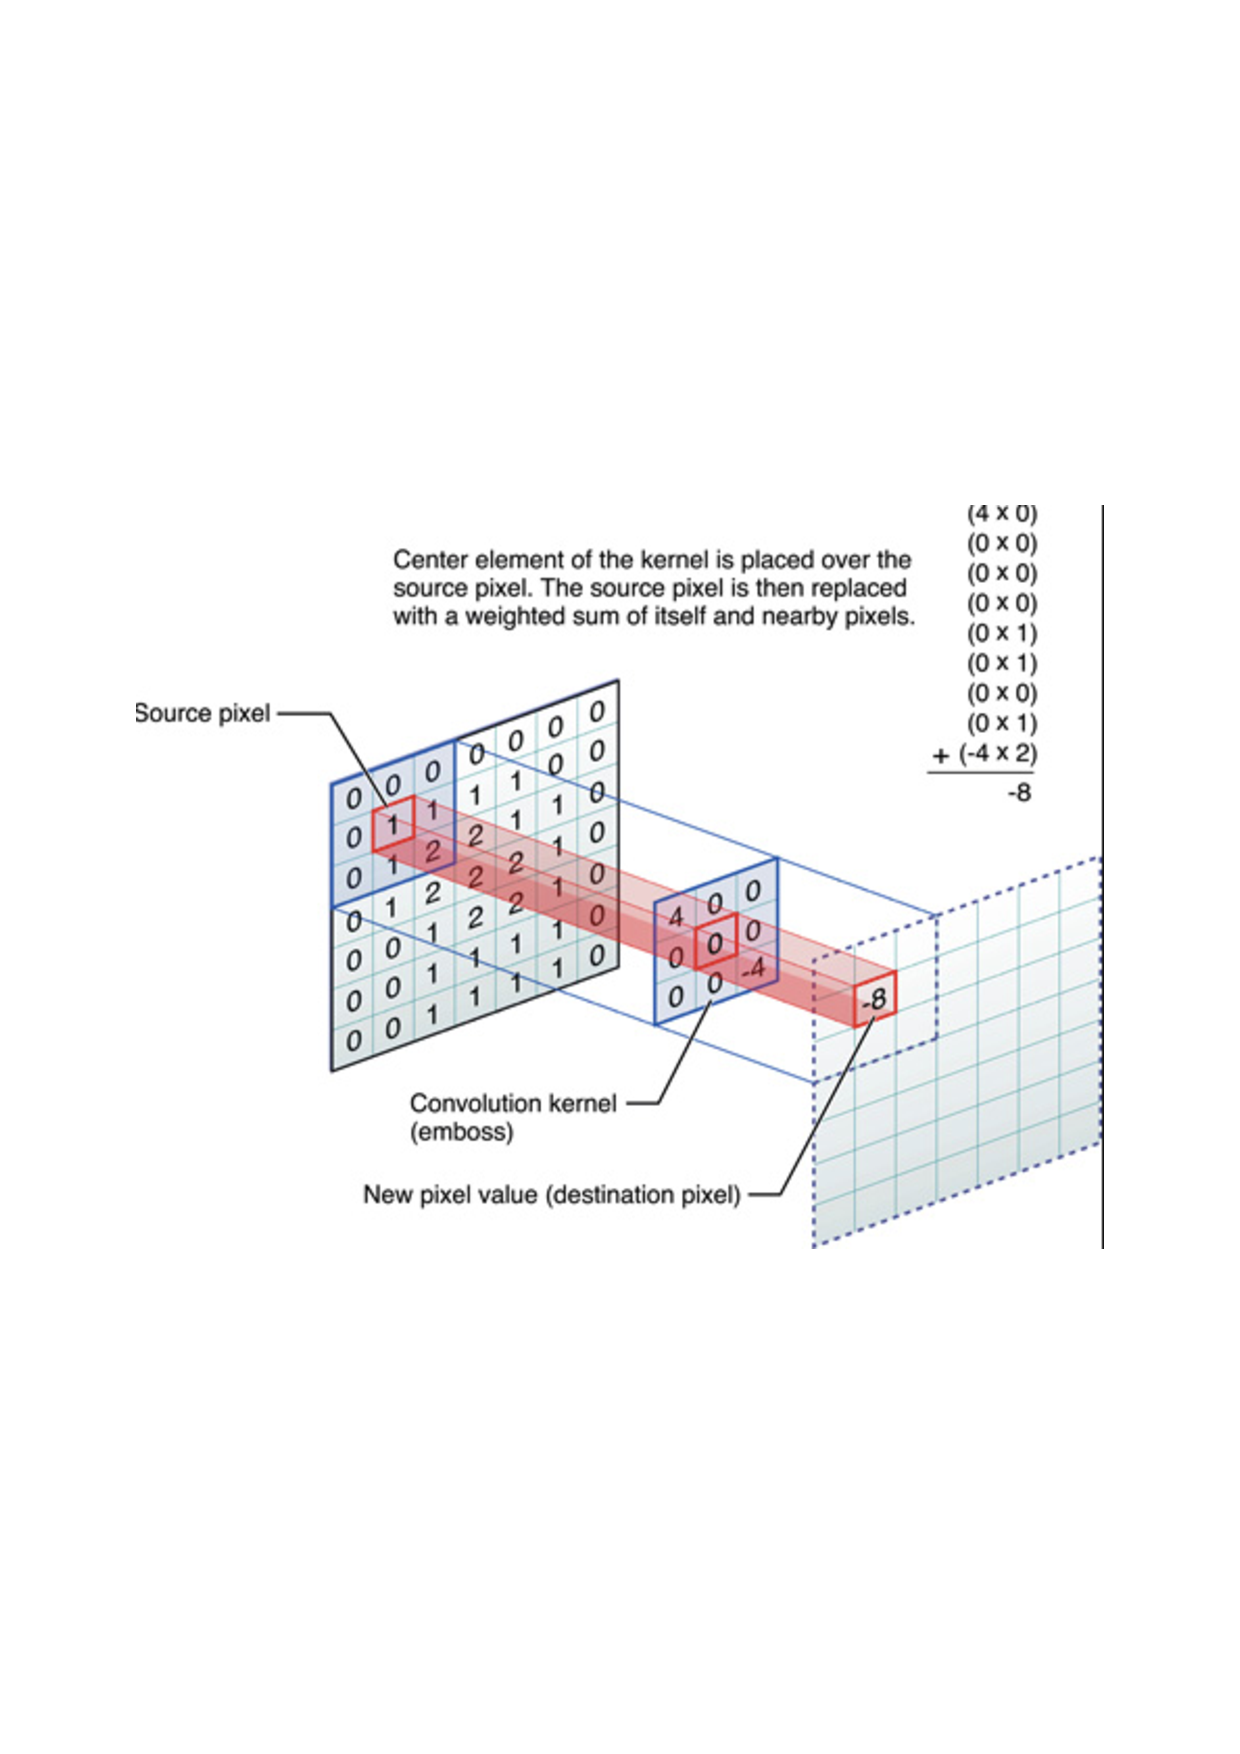
\includegraphics[trim=2cm 7cm 2cm 7cm, clip=true, height=80mm]{Chapter2/convolution.pdf}
\caption{The convolution layer. Illustration of the formation of a feature map.}
\end{figure}

\noindent The benefits of this approach are three folds :

\begin{itemize}
	\item sparse interaction: every output node is connected to a local subset of inputs.
	\item weight sharing: the same kernel, and thus the same set of trainable parameters, is used for every output node to produce a given feature map. 
	\item translational equivariance: shifting the input results in an equivalent shift in the output. This is a property of the convolution operation.
\end{itemize}

\noindent In the detector stage, every node in the feature map is then passed to an nonlinear activation unit thereby introducing non-linearity into the system. These activation units usually consist of either Rectified Linear units (ReLU), Tanh units, or Sigmoid units.\\

\noindent Each feature map is then subsampled in the pooling stage by aggregating contiguous nodes using a summary statistic over a rectangular neighbourhood of outputs. Two commonly used ones are the max and average pooling operations which report respectively the maximum and average of a set of inputs.\\

\noindent The benefits of subsampling are that it reduces the number of features by a factor of k for pooling regions spaced k pixels apart, aiding the classification task and improving the computational efficiency of the network. Furthermore subsampling makes the representation become invariant to small translations of the input. Thus translating the input by a small amount results in little to no change in the values of the pooled outputs.\\

\begin{figure}
\centering
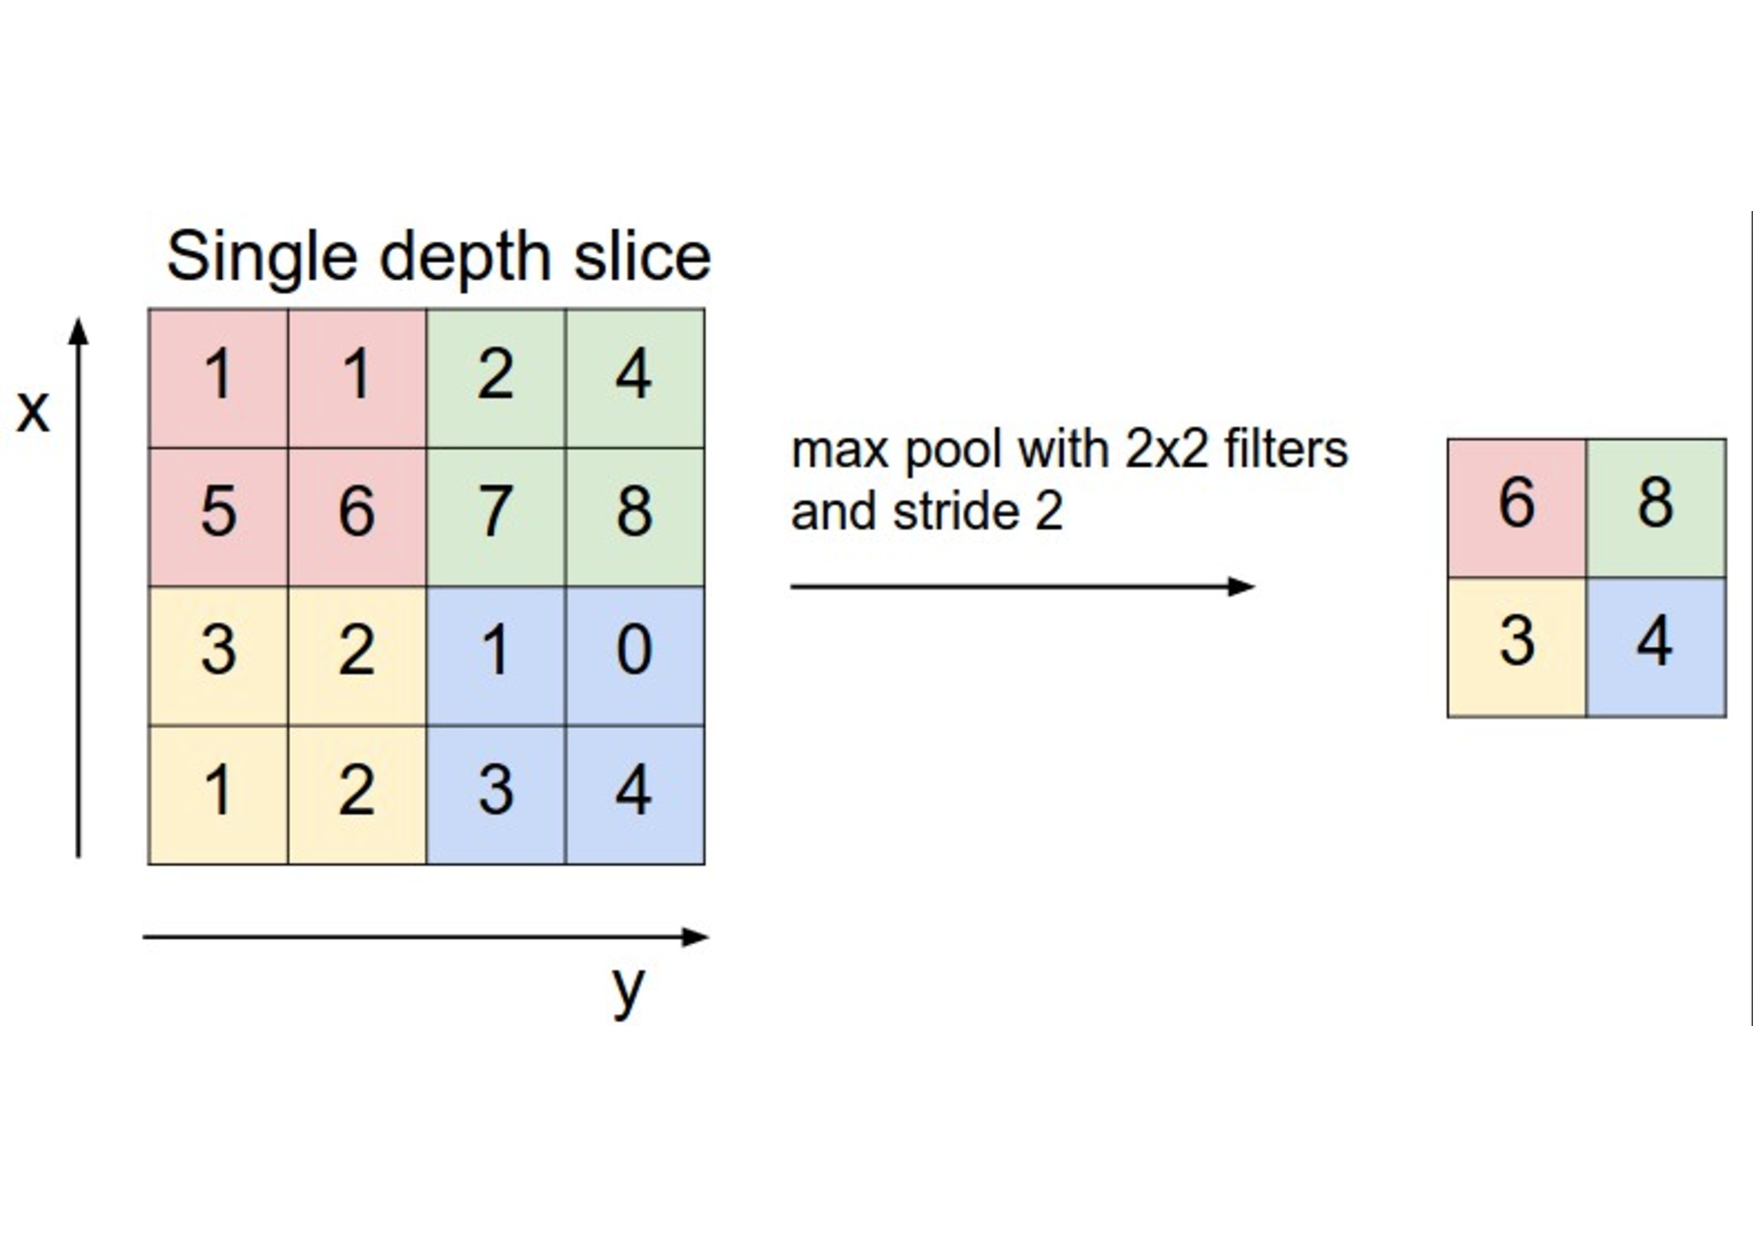
\includegraphics[trim=0cm 0cm 0cm 0cm, clip=true, height=60mm]{Chapter2/pooling.pdf}
\caption{Subsampling in action. Here maxpooling is used to halve the size of an feature map using a $2 \times 2$ filter}
\end{figure}

\subsection{Typical Architecture}

\noindent A typical convolutional neural network architecture consists of an input layer, a number of convolutional layers, a number of fully connected layers, followed by an output layer. The input layer is an $r \times n \times n$ image, with $r$ being the number of channels and $n$ the image height and width. Each channel is passed through a number convolutional layer in parallel. Then the remaining output nodes from all the resulting feature maps across all channels are "flattened" and passed as input to a number of fully connected layers followed by an output layer. The convolutional layers thus serve as a way to reduce the dimensionality of the image by extracting meaningful local features.







